\documentclass[11pt,a4paper]{ctexart}

\usepackage{amsmath,amssymb,bm}
\usepackage{geometry}
\usepackage{enumitem}
\usepackage{fancyhdr}
\usepackage{lastpage}
\usepackage{xcolor}
\usepackage{tcolorbox}
\usepackage{tikz}
\usepackage{titlesec}
\usepackage{microtype}
\usetikzlibrary{arrows.meta,calc,positioning}

\geometry{left=2.15cm,right=2.15cm,top=2.0cm,bottom=2.0cm}
\setlength{\parindent}{2em}
\setlength{\parskip}{0.25em}
\linespread{1.12}

\definecolor{mainblue}{RGB}{39,91,150}
\definecolor{lightblue}{RGB}{232,241,252}
\definecolor{darkgray}{RGB}{65,65,65}
\definecolor{lightgray}{RGB}{245,246,248}

\titleformat{\section}{\large\bfseries\color{mainblue}}{}{0em}{}[\titlerule]
\titleformat{\subsection}{\normalsize\bfseries\color{darkgray}}{}{0em}{}
\titlespacing*{\section}{0pt}{0.9em}{0.45em}
\titlespacing*{\subsection}{0pt}{0.65em}{0.25em}

\setlist[enumerate]{leftmargin=2.2em,itemsep=0.25em,topsep=0.25em}
\setlist[itemize]{leftmargin=2.0em,itemsep=0.2em,topsep=0.2em}

\pagestyle{fancy}
\fancyhf{}
\lhead{\small 格物助航｜每日一练}
\rhead{\small 2026.6.16}
\cfoot{\small 第 \thepage\ 页 / 共 \pageref{LastPage} 页}
\renewcommand{\headrulewidth}{0.4pt}

\newtcolorbox{problemBox}{
  colback=lightblue,
  colframe=mainblue,
  arc=2mm,
  boxrule=0.7pt,
  left=1.0em,
  right=1.0em,
  top=0.8em,
  bottom=0.8em,
  before skip=0.6em,
  after skip=0.8em
}

\newtcolorbox{tipBox}{
  colback=lightgray,
  colframe=darkgray,
  arc=1.5mm,
  boxrule=0.5pt,
  left=0.9em,
  right=0.9em,
  top=0.6em,
  bottom=0.6em,
  before skip=0.5em,
  after skip=0.5em
}

% 自定义命令
\newcommand{\dd}{\mathrm{d}}
\newcommand{\ii}{\bm{i}}
\newcommand{\jj}{\bm{j}}

\begin{document}

\begin{center}
  {\Large\bfseries\color{mainblue} 格物助航｜每日一练}\par
  \vspace{0.25em}
  {\large 电磁学第四章：恒定磁场}\par
  \vspace{0.35em}
  {\small 2026年6月16日}\par
  \vspace{0.35em}
  {\small 编写：谢奕明}
\end{center}

\vspace{-0.3em}

\section*{解题思路提示}
\begin{tipBox}
恒定磁场所涉及的题目通常包括，求磁场和求力。磁场的获得通常有两种方法，对于对称性极高的问题，可以选择\textbf{安培环路定理}简化求解；对于对称性不佳的问题，可能需要利用\textbf{毕-萨定律}结合积分求解。对于求力的问题，则需要使用\textbf{安培力公式}。在求解中，因为要涉及叉乘运算，所以建立适当的坐标系并利用正负表示方向是有必要的。
\end{tipBox}

\section*{习题再现}
\begin{problemBox}
\noindent\textbf{题目 4.17}\quad
如图所示，
\begin{enumerate}
\item[(1)] 一根无限长直导线载有电流 $I_1 = 30\,\text{A}$，矩形回路与它共面，且矩形的长边与直导线平行。回路中载有电流 $I_2 = 20\,\text{A}$，矩形的长 $l = 12\,\text{cm}$，宽 $b = 8.0\,\text{cm}$，矩形靠近直导线的一边距直导线的距离为 $a = 1.0\,\text{cm}$。试求长直导线电流$I_1$的磁场对矩形回路的合力；
\item[(2)] 证明：当矩形线圈足够小时，线圈受到的合力 $F$ 的大小为
\[
F = p_m \frac{\partial B}{\partial x},
\]
其中 $p_m$ 为矩形线圈的磁矩，$\dfrac{\partial B}{\partial x}$ 为直导线产生的磁场沿垂直于直导线方向（图中 $x$ 方向）上的磁场梯度。
\end{enumerate}

\vspace{0.8em}
\begin{center}
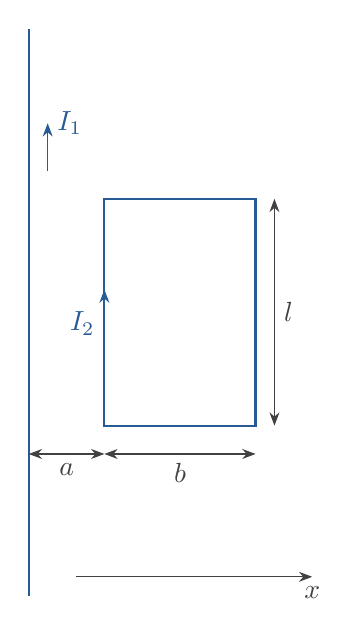
\begin{tikzpicture}[>=Stealth, scale=1.2]
    \definecolor{mainblue}{RGB}{39,91,150}
    
    % 无限长直导线（竖直）
    \draw[thick, mainblue] (0,-3) -- (0,3);
    \draw[->, mainblue] (0.2,1.5) -- (0.2,2.0) node[right] {$I_1$};
    
    % x 轴方向示意
    \draw[->, darkgray] (0.5,-2.8) -- (3,-2.8) node[below] {$x$};
    
    % 矩形回路尺寸（相对比例）
    \def\a{0.8}      % 距离 a
    \def\b{1.6}      % 宽度 b
    \def\l{2.4}      % 长度 l
    \coordinate (A) at (\a, -1.2);
    \coordinate (B) at (\a+\b, -1.2);
    \coordinate (C) at (\a+\b, 1.2);
    \coordinate (D) at (\a, 1.2);
    \draw[thick, mainblue] (A) -- (B) -- (C) -- (D) -- cycle;
    
    % 只在左边框标注电流方向向上
    \draw[->, mainblue] ($(A)!0.3!(D)$) -- ($(A)!0.6!(D)$) node[midway, left] {$I_2$};
    
    % 尺寸标注 a 和 b（同一高度，y = -1.5）
    \draw[<->, darkgray] (0, -1.5) -- (\a, -1.5) node[midway, below] {$a$};
    \draw[<->, darkgray] (\a, -1.5) -- (\a+\b, -1.5) node[midway, below] {$b$};
    
    % 标注长边 l
    \draw[<->, darkgray] (\a+\b+0.2, -1.2) -- (\a+\b+0.2, 1.2) node[midway, right] {$l$};
\end{tikzpicture}
\end{center}
\end{problemBox}

\section*{详细解法}

\subsection*{(1) }

对于无限长直导线，电流 \(I\) 沿轴线方向，磁场具有轴对称性。取以导线为轴、半径为 \(x\) 的圆形环路，环路平面与导线垂直。由于磁场方向沿切线，大小 \(B\) 在环路上恒定，得：
\[
B \cdot 2\pi x = \mu_0 I_1 .
\]
所以
\[
B(x) = \frac{\mu_0 I_1}{2\pi x},
\]
在图中线框一侧，磁场方向垂直纸面向里。利用毕-萨定律也可以得到这个结果（读者可以复习）。

矩形回路由四段组成，分别计算安培力：

\begin{itemize}
\item \textbf{左边段（靠近直导线，距 $x=a$）}：电流方向向上，根据安培力公式 $\boldsymbol{F}=I_2 \boldsymbol{l} \times \boldsymbol{B}$，受力方向水平向左，大小为
\[
F_{\text{左}} = I_2 \cdot l \cdot B(a) = I_2 l \cdot \frac{\mu_0 I_1}{2\pi a}.
\]

\item \textbf{右边段（距 $x=a+b$）}：电流方向向下，受力方向水平向右，大小为
\[
F_{\text{右}} = I_2 l \cdot B(a+b) = I_2 l \cdot \frac{\mu_0 I_1}{2\pi (a+b)}.
\]

\item \textbf{上边段和下边段}：由于磁场方向垂直纸面，而电流方向为水平，故安培力方向竖直。上边段各点的磁场大小随 $x$ 变化，但由对称性，上下两段所受的竖直方向力大小相等、方向相反，相互抵消。因此合力只考虑左右两段水平方向的贡献。
\end{itemize}
合力方向水平向左，大小为
\[
F = F_{\text{左}} - F_{\text{右}} = \frac{\mu_0 I_1 I_2 l}{2\pi} \left( \frac{1}{a} - \frac{1}{a+b} \right).
\]
代入数据
$
\mu_0 = 4\pi \times 10^{-7}\,\text{N/A}^2,\quad
I_1 = 30\,\text{A},
I_2 = 20\,\text{A},
l = 0.12\,\text{m},
a = 0.01\,\text{m},
b = 0.08\,\text{m}
$
得
\[
F = \frac{(4\pi \times 10^{-7}\,\text{N/A}^2) \times (30\,\text{A}) \times (20\,\text{A}) \times (0.12\,\text{m})}{2\pi} \left( \frac{1}{0.01\,\text{m}} - \frac{1}{0.09\,\text{m}} \right) = 1.28 \times 10^{-3}\,\text{N}.
\]
所以合力大小为 $1.28\times10^{-3}\,\text{N}$，方向指向直导线。

\subsection*{(2) }

当矩形线圈足够小时（即 $b \ll a$，线圈的宽度远小于到直导线的距离），可认为线圈所在区域的磁场近似线性变化。将 $B(a+b)$ 在 $x=a$ 处泰勒展开：
\[
B(a+b) \approx B(a) + \left.\frac{\dd B}{\dd x}\right|_{x=a} \cdot b.
\]
合力表达式变为（正负表示方向）：
\[
F = - I_2 l B(a)  + I_2 l B(a+b) \approx I_2 l \left[ - B(a) + \left( B(a) + \frac{\dd B}{\dd x} b \right) \right] = I_2 l b \frac{\dd B}{\dd x}.
\]
尽管本题中磁场是$x$的一元函数，但为了更具一般性，我们把导数改为偏导数，表示磁场可能还与其他空间坐标有关，即：
\[
F = I_2 l b\frac{\partial B}{\partial x}.
\]
线圈的磁矩大小为 $p_m = I_2 \cdot S = I_2 \cdot l b$。故有
\[
F = p_m \frac{\partial B}{\partial x}.
\]
方向沿 $−x$ 方向，即指向长直导线。证毕。

\section*{技巧与知识点}
\begin{tipBox}
\begin{itemize}
  \item \textbf{毕奥—萨伐尔定律}：\(\displaystyle \dd\boldsymbol{B} = \frac{\mu_0}{4\pi} \frac{I\dd\boldsymbol{l} \times \hat{\boldsymbol{R}}}{R^2}\)。
  \item \textbf{安培环路定理}：\(\displaystyle \oint \boldsymbol{B} \cdot \dd\boldsymbol{l} = \mu_0 I_{\text{enc}}\)。
  \item \textbf{安培力公式}：\(d \boldsymbol{F}=I d \boldsymbol{l}\times\boldsymbol{B}\)。
  \item \textbf{磁矩}：\(\displaystyle \boldsymbol{p}_m = I \boldsymbol{S}\)，大小 \(p_m = I \cdot (\text{面积})\)。
\end{itemize}
\end{tipBox}

\section*{复习建议}
\begin{tipBox}
恒定磁场解题核心：
\begin{enumerate}
  \item \textbf{求磁场}：面对对称分布的磁场，可以用安培环路定理（无限长直导线、螺线管、环形螺线管等）；非对称则用毕奥—萨伐尔定律再积分获得，注意系数正确。
  \item \textbf{求安培力}：载流导线受力 \( d \boldsymbol{F}=I d \boldsymbol{l}\times\boldsymbol{B}\)；匀强磁场中直导线：\(F=IlB\sin\theta\)。
  \item \textbf{求磁矩}：线圈磁矩 \(\boldsymbol{p}_m=I\boldsymbol{S}\)，对任意形状均如此。
  \item \textbf{洛伦兹力}：运动电荷受力 \(\boldsymbol{F}=q\boldsymbol{v}\times\boldsymbol{B}\)，用于求解带电粒子在均匀磁场中的运动问题。
  \item \textbf{方向的判断}：可以用高中阶段所学的左右手定则，不过熟记公式并用右手确定叉乘的方向也很迅速。对于比较复杂的问题，一定不要逞强，建议踏踏实实建好坐标系，用坐标分量的正负来判断方向。
\end{enumerate}
\end{tipBox}
\end{document}